\section{Actividad No 01 – Conectar a SQL Server desde Power BI Desktop} 



\begin{enumerate}[1.]
	\item  En el cuadro de dialogo base de datos SQL Server, en la casilla servidor tipear (local), en la casilla Base de datos (opcional) / Database (optional), tipear AdventureWorks2017, y hacer clic en OK.
	

	\begin{center}
	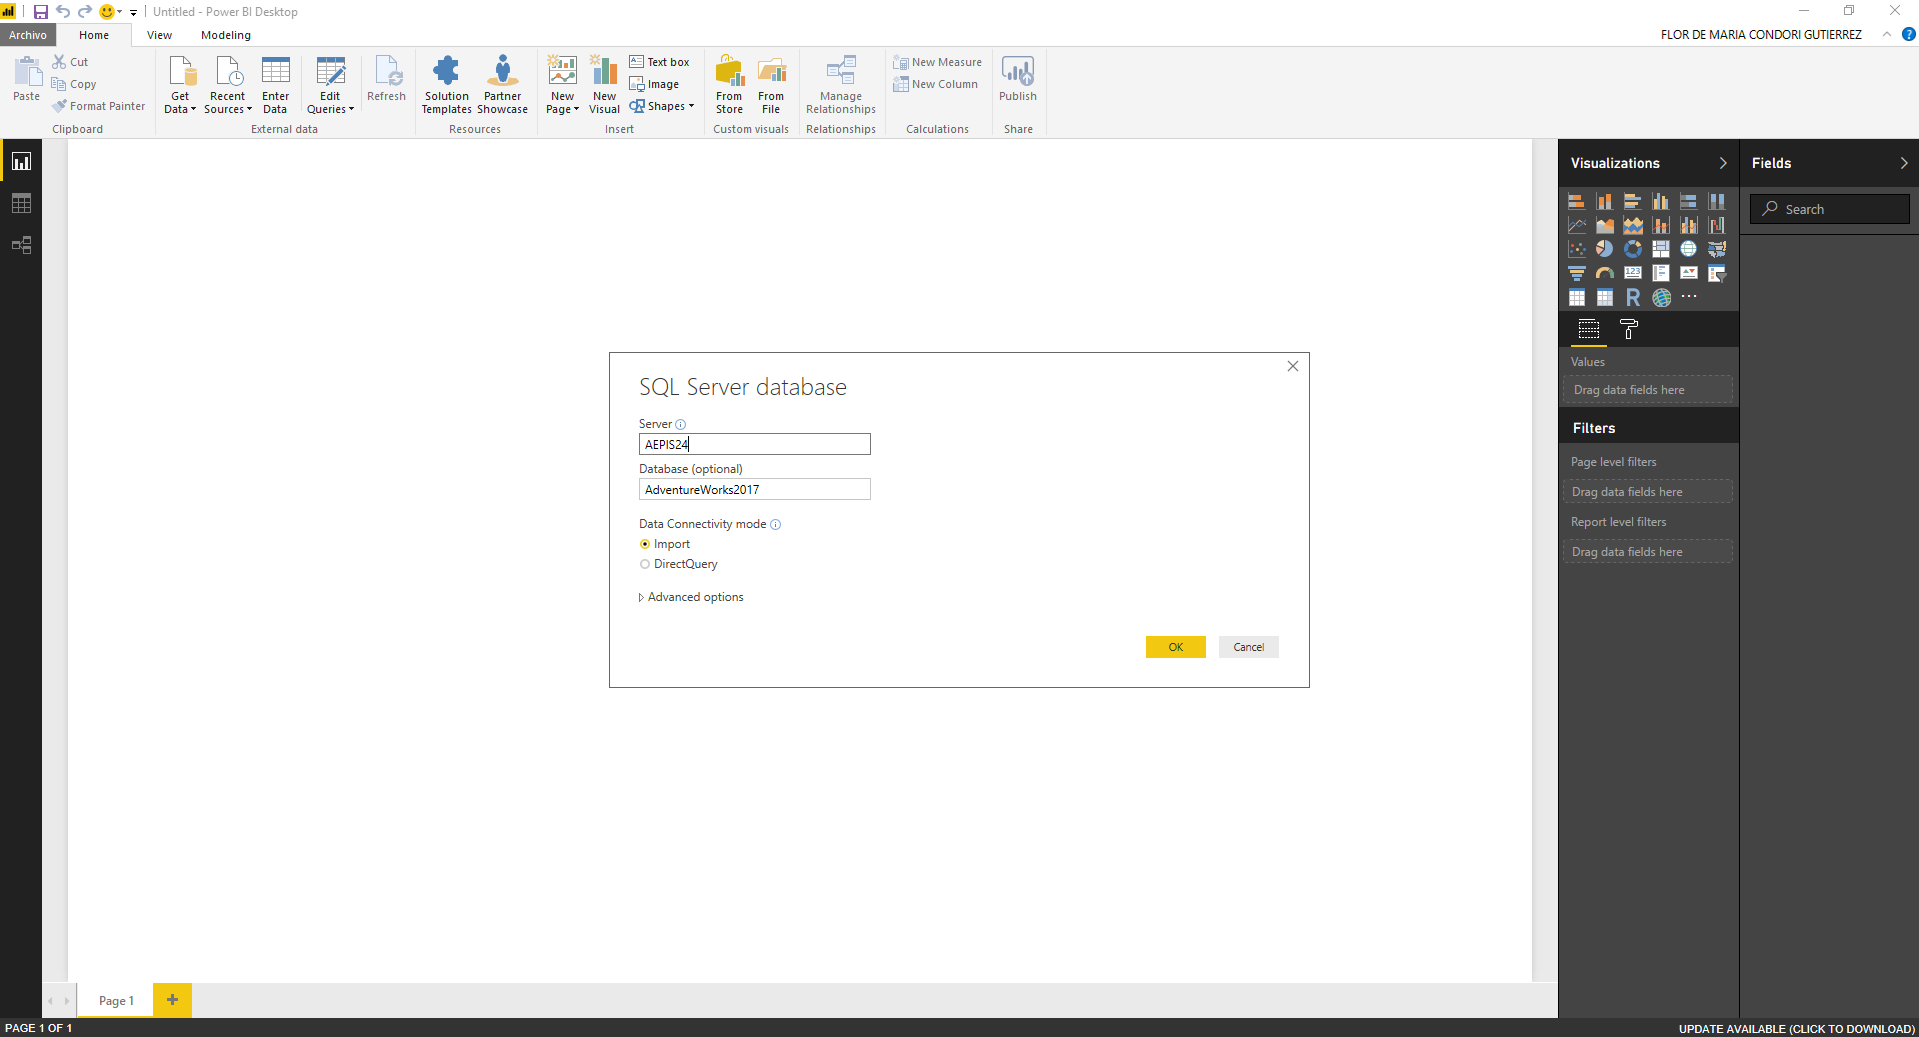
\includegraphics[width=16cm]{./Imagenes/11} 
	\end{center}


	\item  En el cuadro de dialogo Navegador (Navigator), seleccionar el check en Sales.vSalesPerson, y entonces hacer click en Cargar (Load).

	\begin{center}
	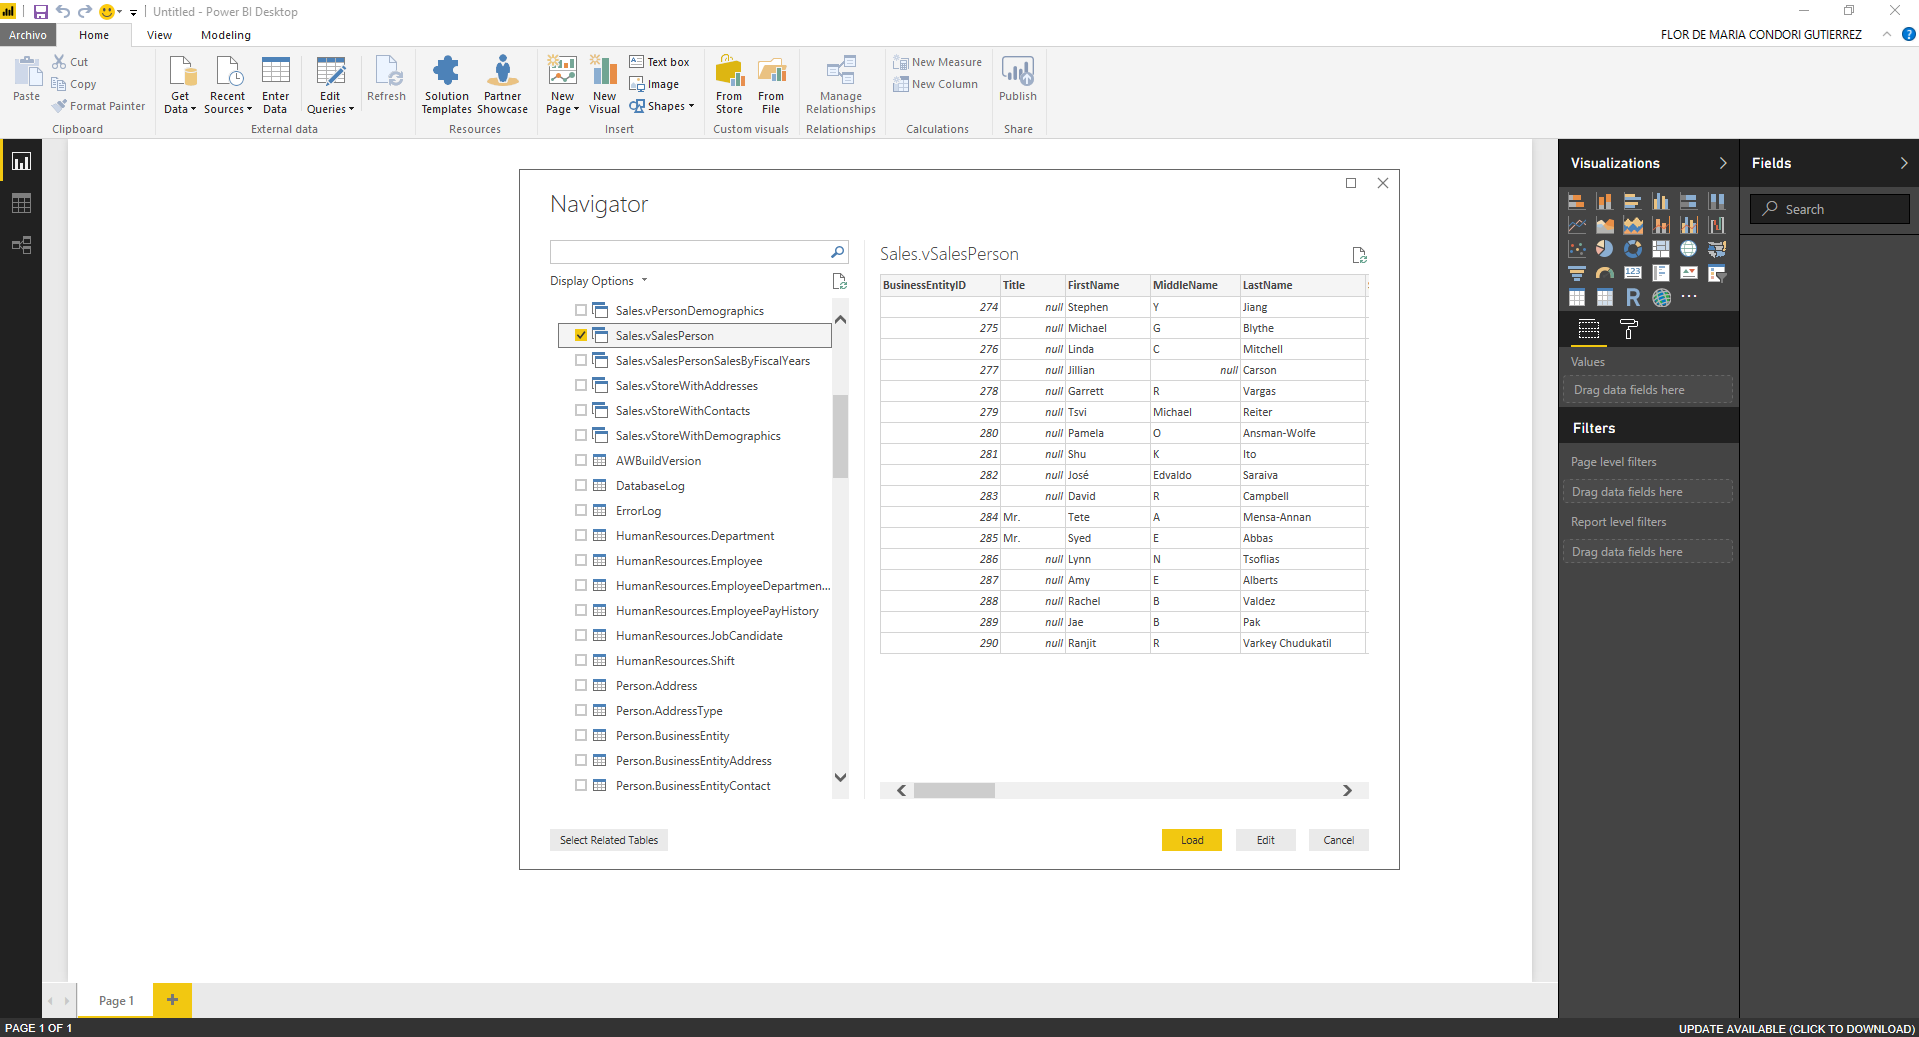
\includegraphics[width=16cm]{./Imagenes/12} 
	\end{center}


	\item Expandir opciones Avanzadas, en la casilla sentencia SQL (opcional, base de datos requerida), tipear la siguiente consulta, y luego hacer click en OK:
	\\
	\\SELECT TOP 10 P.ProductID, P.Name AS Product, SUM(CAST(LineTotal AS decimal(18,2))) AS LineTotal FROM 	Purchasing.PurchaseOrderDetail AS POD INNER JOIN Production.Product AS P ON POD.ProductID = P.ProductID GROUP BY P.ProductID, P.Name ORDER BY LineTotal DESC

	\begin{center}
	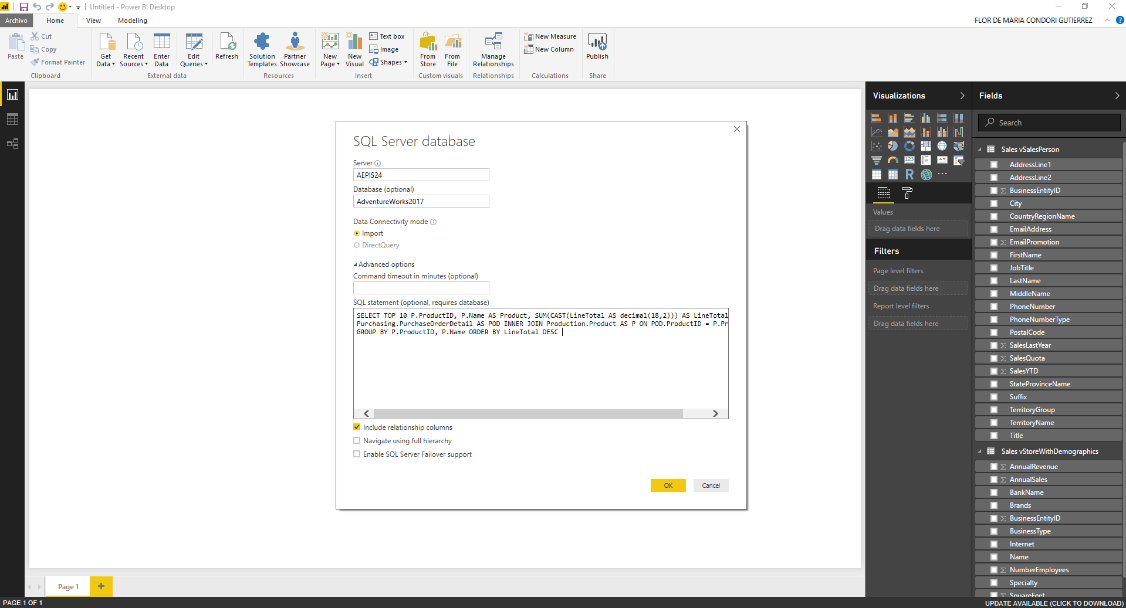
\includegraphics[width=16cm]{./Imagenes/13} 
	\end{center}

\end{enumerate}




